\documentclass{article}
\usepackage[usenames,dvipsnames]{xcolor}
\usepackage{nips10submit_e,times}
\usepackage{algpseudocode}
%\documentstyle[nips07submit_09,times]{article}
\usepackage[square,numbers]{natbib}
\usepackage{amsmath, epsfig}
\usepackage{amsfonts}
\usepackage{subfigure}
\usepackage{graphicx}
\usepackage{amsfonts}
\usepackage{algorithm}
\usepackage{easybmat}
\usepackage{footmisc}
\renewcommand\algorithmiccomment[1]{// \textit{#1}}
%
\newcommand{\ignore}[1]{}
\newcommand{\comment}[1]{}
\DeclareMathOperator*{\argmax}{arg\,max}

\title{Semi-Supervised Multidimensional Personal Emotion Classification}

\author{
Kui Tang\\
Columbia University, New York, NY 10027, USA\\
\texttt{\{kt2384\}@columbia.edu},
}

% The \author macro works with any number of authors. There are two commands
% used to separate the names and addresses of multiple authors: \And and \AND.
%
% Using \And between authors leaves it to \LaTeX{} to determine where to break
% the lines. Using \AND forces a linebreak at that point. So, if \LaTeX{}
% puts 3 of 4 authors names on the first line, and the last on the second
% line, try using \AND instead of \And before the third author name.

\newcommand{\fix}{\marginpar{FIX}}
\newcommand{\new}{\marginpar{NEW}}
\newcommand{\X}{\mathcal{X}}

\nipsfinalcopy

\begin{document}

\maketitle

\begin{abstract}
Modelling emotional data is a relatively immature field. Most
approaches focuses on \emph{sentiment analysis}, a binary (negative
or positive) classification of emotion. Moreover, most applications
only care about aggregating of global sentiment, ignoring sentiments
of individual users.  Applications in human-computer interaction
and recommendation systems for web applications can benefit from
the machine's knowledge of the particular user's emotional state.
However, high quality mutimodal labelled corpora are difficult to
find. In this project, we derive a personal emotional lexicon from
Tumblr blogs, data sources rich in emotional content. We take a
semi-supervised approach with latent Dirichlet allocation (LDA) and
a derivative, SubjLDA, initializing our model with labelled emotional
words with a small non-domain-specific lexicon and allowing the
model to classify the remaining words and documents into emotional
categories.
\end{abstract}

\section{Introduction}
\begin{quote}
It is obvious, that when we have the prospect of pain or pleasure
from any object, we feel a consequent emotion of aversion or
propensity, and are carryed to avoid or embrace what will give us
this uneasines or satisfaction. \ldots Here then reasoning takes
place to discover this relation; and according as our reasoning
varies, our actions receive a subsequent variation. But it is evident
in this case that the impulse arises not from reason, but is only
directed by it.

\hspace{9 cm} --- Hume \citep{hume}
\end{quote}
As a person is ultimately driven to action based on emotion, 

\label{sec:introduction}

\subsection{Related Work}
The explosion of social media---particularly (micro)blogs, product
reviews, and recommendations---drives both demand and opportunity
for mining sentiments from text. Early work by Turney in 2002
\citep{turney02} uses an unsupervised method of computing \emph{pointwise
mutual information} between words in product reviews with the seed
words ``excellent'' and ``poor''. Indeed, most work, including the
model on which this project is based \citep{lin03}, models emotion
as a one-dimensional continuum between positive and negative.

We thus move to multidimensional emotional analysis. Rather than
start with merely two mood states, multidimensional analyses begin
with lists of seed words for each emotional dimension of interest.
The earliest standard lexicon is the the art is the \emph{Profile
of Mood states} \citep{mcnair71}, a psychological survey that
includes 65 items labelled across six distinct states. Bollen et
al. extend this list to a lexicon of 964 terms by adding co-related
words appearing in Google's n-gram data and use this data to regress
DJIA closing prices against a time series of aggregate inferred
Twitter sentiment \citep{bollen11}. They find more significant
Granger-causality p-values in a lag of 2--6 days when incorporating
a multidimensional lexicon compared to significance only in one-day
lags on a unidimensional lexicon. The WordNet-Affect project begins
with a seed list of manually curated terms, and then iteratively
finds synsets with WordNet to expand the list \citep{strapparava04}.
In this project we use WordNet-Affect data as our priors.

Texts do not generally come with explicit emotional tags, so
supervised techniques have limited scope. One notable exception is
Livejournal, which allows users to specify one of 142 distinct moods
when composing a blog post. Mishne et. al \citep{mishne06} use these
labels to build a linear regression model, predicting mood
\emph{levels}---the sum of mood tags at a given hour---from total
post intensity, hour of the day, and frequencies of individual
terms. Sood and Vasserman use k-means to compactify the set of 142
mood descriptors into just 3 (happy, sad, angry) and apply Naive Bayes
with the new labels.

Finally, \emph{supervised LDA} models document classification onto
predefined labels as a regression problem with a categorical response.
Blei et al. show an improvement in per-word likelihood on movie reviews
and Digg data compared to LDA.~\citep{blei07}.

\section{Problem Description}
The above work handles on \emph{aggregate} sentiment analysis, which
is great for marketing and stock trading, but less applicable to
\emph{affective computing}. Rosalind~\citep{picard97} argues that because emotions
are essential to human reasoning, learning, and pattern recognition,
if we wish to develop more natural, human-like behavior in machines,
we must equip machines with emotional intelligence.
A basic problem which we confront in this project is to learn a
user's emotional state from text. Only with knowledge of how a user
feels can machines produce emotionally intelligent responses.

Given a set of blog posts from one user, we wish to infer a
personalized, probabilistic lexicon of emotion. Certain words such
as `love' and `fear' clearly signifiy a particular emotion.  However,
manually curated lexica are sparse, and each person uses language
in a slightly different way and carries unique connotations. A
medical student write about her work experiences at the hospital,
thereby associating the word `hospital' with aspiration and career
success. But most people associate hospitals with fear and uncertainty.
Thus, in a similar situation as speech recognition, applications
that attempt to infer the user's emotional state should improve
their performance when trained user-specific data.

In this project, we start with a small, hand-labelled lexicon of
emotional words as a baseline. We compare this baseline against two
topic models adapted for emotional classification to show a performance
increase after training on user-specific texts.

\section{Models}
\subsection{Latent Dirichlet Allocation}
Latent Dirichlet allocation~\citep{blei03} models each document $d$
(here, a blog post) as a multinomial distribution $\theta_d$ over
a sparse subset of latent topics $Z$.  Each index $i$ in a document
is drawn from this multinomial topic distribution, giving each word
a topic label $z_i^d$. Conditioned on this topic label, a word
$w_i^d$ is drawn from a multinomial distribution $\beta_{z_i^d}$.
Here, we fix the number of topics to 7 to include the six emotions
in our prior lexicon plus a neutral emotion. We implement the
standard collapsed Gibbs sampler.

\subsection{SubjLDA} \label{sec:subjlda}
SubjLDA is a model by Lin~\citep{lin03} which adds a sentence-level
subjectivity latent variable. Each sentence is either objective or
subjective. Conditioned on subjectivity, a sentiment label is drawn
for each word in that sentence. Since a single document can shift
emotions, the sentence-level hierarchy allows this model to better
capture local sentiment. The generative procedure for SubjLDA
follows:

\begin{enumerate}
\item For each sentiment label $l$:
\begin{enumerate}
\item Draw $\mathbf{\phi}_l \sim \mbox{Dir}(\mathbf{\lambda}_l \cdot \mathbf{\beta}_l)$, a multinomial distribution over words for the sentiment label $l$.
\end{enumerate}
\item For each document $d$:
\begin{enumerate}
\item Draw $\mathbf{\pi}_d \sim \mbox{Dir}(\gamma)$, a multinomial distribution over subjectivity labels for each sentence in document $d$.
\item For each sentence $j$:
\begin{enumerate}
\item Draw a subjectivity label $s_{d,j} \sim \mbox{Multinomial}(\mathbf{\pi}_d)$
\item Draw a $\mathbf{\theta}_{d,m} \sim \mbox{Dir}(\mathbf{\alpha_{s_{d,m}}})$, a distribution of sentiments for sentence $j$ of document $d$. 
\item For each $N_{d,m}$ word position in sentence $m$ of document $d$
\begin{enumerate}
\item Draw a sentiment $l_{d,m,t} \sim \mbox{Mult}(\mathbf{\theta}_{s_{d,m}})$
\item Draw a word $w_{d,m,t} \sim \mbox{Mult}(\mathbf{\phi}_{l_{d,m,t}})$
\end{enumerate}
\end{enumerate}
\end{enumerate}
\end{enumerate}

Each $\mathbf{\alpha}$ encodes an asymmetric Dirichlet prior on the
distributions of sentiments given a subjectivity. In our inference,
we initialize our labels with a training corpus, and use a
maximum-likelihood estimate for $\mathbf{\alpha}$, computed using
a Newton-Raphson iteration from the initializing sentiment and
subjectivity labels~\citep{minka00}. Each $\mathbf{\beta}$ is
scaled to the empirical frequency of training words for each
sentiment. The prior $\gamma$ controls the mixing coefficients of
subjectivity labels (subjective or objective). Thus, our priors
capture the asymmetry of sentiment: that objective and subjective
sentences are not equally prevalent, that most words are neutral,
and that words may nobe be distributed uniformly across emotions.
Further details on these priors below.

Let $\mathbf{w}$ denote a bag-of-words vector of words, $\mathbf{s}$
denote a vector of subjectivity labels, and $\mathbf{l}$ denote a vector
of sentiment labels. Then the joint distribution is
\begin{equation}
\begin{aligned}
P(\mathbf{w,s,l}|\mathbf{\alpha,\beta,\gamma}) &= P(\mathbf{w}|\mathbf{l,\beta})P(\mathbf{l}|\mathbf{s,\alpha})P(\mathbf{s}|\mathbf{\gamma}) \\
    &= \int P(\mathbf{w}|\mathbf{l,\beta})P(\mathbf{l}|\mathbf{\beta}) d\Phi \int P(\mathbf{l}|\mathbf{\Theta})P(\mathbf{\Theta}|\mathbf{s,\alpha})d\Theta \int P(\mathbf{s}|\mathbf{\Pi})P(\mathbf{\Pi}|\mathbf{\gamma}) d\mathbf{\Pi}
\end{aligned}
\end{equation}

We can analytically integrate out the parameters to get conditional
distributions for each sentiment and subjectivity label and thus
build a Gibbs sampler. For details, see~\citep{lin03}.

\subsection{Priors}
We follow Lin's approach to implement semi-supervised learning via
empirical Bayes, initializing the latent variables and model priors
using existing corpora. We use the words under the {\sc emotion}
label in WordNet-Affect 1.0 \citep{strapparava04}, which provides
606 words labelled with one of ``anger'', ``disgust'', ``fear'',
``joy'', ``sadness'', ``surprise''. We also used the neutral words
from SentiWordNet~\citep{baccianella10}, the same source as Lin.

For each word in the training set, if we found that word in either
prior lexicon, we set the appropriate sentiment label. If a sentence
contained any non-neutral words, we labelled that sentence subjective.
Otherwise, we labelled the sentence objective.

If a word was not matched by emotion or neutrality (rare; less than
10\%) of the time, we randomly assigned it an emotion.

The majority of words were neutral. Of 286,997 words in the 
poetry blog, 240,087, or 83.6\%, were discovered to be neutral.

\section{Data}
Data were scraped from Tumblr in April 2012. The API
was not usable because it only allowed access to users who have
authenticated the API key for this application. However, as this
model works on only a single user's blog, applications could work
over the API.

Not all Tumblr sites shared the same HTML layout, but upon inspection
of the source codes, a small number of XPath queries were able to
extract all textual content.  Parsing and text extraction was
performed with lxml.

For these results, we analyzed three blogs, consisting mainly of
personal writings in politics, prose, and poetry. All posts were
by the same user---a critical feature of our model.

\begin{table} 
\centering
\begin{tabular}{ l l c c c }
\bf URL & \bf Genre & \bf Posts & \bf Words & \bf Vocabulary \\
\hline
thenatureofdaylight.tumblr.com & poetry & 1,325 & 88,664 & 8,973 \\
noconsensusonaname.tumblr.com & prose & 288 & 26,090 & 5,958 \\
pantslessprogressive.com & politics & 4,736 & 360,886 & 28,592 \\
\end{tabular}
\caption{Sizes of our data sets, after stemming and removing stopwords and short posts.\label{tab:data}}
\end{table}

To limit ourselves to ``important'' posts, we dropped all posts
with fewer than 20 words. We randomly chose 20\% of posts to hold
as a test set to evaluate our model's performance

\subsection{Feature Extraction}
Both LDA and SubjLDA represent the document as a bag of words.  In
addition, SubjLDA requires identifying sentences in documents, as
it posits that sentences are associated with distinct distributions
of sentiment.

To parse the data into sentences and words, we used the standard
Punkt sentence tokenizer in NLTK~\citep{bird09}. To reduce data
sparsity, we ran the Porter stemmer and removed stemmed stopwords.

\section{Results} 
A simple single-core Python implementation of Gibbs sampling for
SubjLDA processed on average 2,715.8 words per second, which comes
to 26.0 seconds per iteration for the poetry blog of 1036 posts.
For each of the three blogs (politics, prose, poetry), we ran 400
Gibbs sampling iterations overnight on an eight-core Amazon EC2
high-CPU instance. The largest dataset, pantslessprogressive.com,
took 24 hours to reach 400 iterations. Had there been more time,
we would have diagnosed convergence to determine the necessary
number of iterations.

\subsection{Highly Probable Words}
\begin{table}
\centering
\begin{tabular}{ l l l l l l l  }
\multicolumn{7}{c}{ \sc SubjLDA on thenatureofdaylight.tumblr.com }\\
\sc neutral & \sc anger & \sc disgust & \sc fear & \sc joy & \sc sadness & \sc surprise \\
\hline
life & re & redrum & n't & \textcolor{ForestGreen}{\textbf{love}} & n't & ask \\
one & \textcolor{BrickRed}{\textbf{get}} & sourc & \textcolor{BrickRed}{\textbf{like}} & \textcolor{ForestGreen}{\textbf{like}} & know & \textcolor{BrickRed}{\textbf{friend}} \\
time & \textcolor{BrickRed}{\textbf{look}} & day & ca & \textcolor{ForestGreen}{\textbf{give}} & m & anonym \\
thing & fuck & jonathan & want & would & \textcolor{BrickRed}{\textbf{like}} & \textcolor{ForestGreen}{\textbf{get}} \\
want & make & grow & \textcolor{BrickRed}{\textbf{live}} & everyth & \textcolor{ForestGreen}{\textbf{feel}} & know \\
never & \textcolor{BrickRed}{\textbf{good}} & \textcolor{BrickRed}{\textbf{enjoy}} & question & alway & even & \textcolor{BrickRed}{\textbf{like}} \\
think & say & definit & \textcolor{ForestGreen}{\textbf{away}} & \textcolor{ForestGreen}{\textbf{look}} & go & best \\
everi & n't & fight & oh & \textcolor{ForestGreen}{\textbf{live}} & \textcolor{ForestGreen}{\textbf{sad}} & re \\
\textcolor{BrickRed}{\textbf{feel}} & guy & bridg & \textcolor{BrickRed}{\textbf{dark}} & make & miss & n't \\
     peopl & \textcolor{ForestGreen}{\textbf{hate}} & perhap & promis & person & \textcolor{BrickRed}{\textbf{pleas}} & girl \\
\multicolumn{7}{c}{ } \\
\multicolumn{7}{c}{ \sc LDA on thenatureofdaylight.tumblr.com }\\
\sc neutral & \sc anger & \sc disgust & \sc fear & \sc joy & \sc sadness & \sc surprise \\
\hline
n't & \textcolor{ForestGreen}{\textbf{see}} & redrum & \textcolor{ForestGreen}{\textbf{away}} & \textcolor{ForestGreen}{\textbf{love}} & fog & wind \\
    \textcolor{BrickRed}{\textbf{like}} & fuck & \textcolor{BrickRed}{\textbf{love}} & \textcolor{BrickRed}{\textbf{heart}} & life & fuck & cock \\
    want & \textcolor{BrickRed}{\textbf{love}} & \textcolor{BrickRed}{\textbf{away}} & \textcolor{BrickRed}{\textbf{air}} & \textcolor{ForestGreen}{\textbf{give}} & \textcolor{BrickRed}{\textbf{along}} & rose \\
    know & \textcolor{ForestGreen}{\textbf{hate}} & region & \textcolor{ForestGreen}{\textbf{shadow}} & \textcolor{ForestGreen}{\textbf{heart}} & bus & stand \\
    one & amp & link & \textcolor{BrickRed}{\textbf{like}} & \textcolor{BrickRed}{\textbf{see}} & \textcolor{ForestGreen}{\textbf{tear}} & templ \\
    m & reggi & everyon & \textcolor{BrickRed}{\textbf{see}} & \textcolor{ForestGreen}{\textbf{live}} & hors & \textcolor{BrickRed}{\textbf{heart}} \\
    time & tito & \textcolor{BrickRed}{\textbf{scene}} & color & \textcolor{BrickRed}{\textbf{tear}} & \textcolor{BrickRed}{\textbf{away}} & begin \\
    \textcolor{BrickRed}{\textbf{feel}} & line & book & sourc & \textcolor{BrickRed}{\textbf{away}} & lost & \textcolor{BrickRed}{\textbf{air}} \\
    thing & \textcolor{ForestGreen}{\textbf{red}} & point & paint & \textcolor{ForestGreen}{\textbf{scream}} & \textcolor{BrickRed}{\textbf{like}} & dead \\
    would & lyric & \textcolor{BrickRed}{\textbf{short}} & band & \textcolor{ForestGreen}{\textbf{inspir}} & chandeli & \textcolor{ForestGreen}{\textbf{get}} \\
\multicolumn{7}{c}{ } \\
\multicolumn{7}{c}{ \sc SubjLDA on noconsensusonaname.tumblr.com }\\
\sc neutral & \sc anger & \sc disgust & \sc fear & \sc joy & \sc sadness & \sc surprise \\
\hline
one & cours & \textcolor{BrickRed}{\textbf{like}} & someth & \textcolor{ForestGreen}{\textbf{like}} & would & n't \\
know & \textcolor{ForestGreen}{\textbf{short}} & would & tri & \textcolor{ForestGreen}{\textbf{look}} & want & \textcolor{ForestGreen}{\textbf{get}} \\
could & believ & \textcolor{ForestGreen}{\textbf{turn}} & \textcolor{ForestGreen}{\textbf{away}} & n't & everyth & re \\
go & began & never & \textcolor{BrickRed}{\textbf{emot}} & fuck & \textcolor{ForestGreen}{\textbf{dark}} & anyth \\
make & lie & mouth & import & \textcolor{ForestGreen}{\textbf{live}} & \textcolor{BrickRed}{\textbf{expect}} & \textcolor{BrickRed}{\textbf{good}} \\
back & cool & d & mayb & \textcolor{ForestGreen}{\textbf{move}} & \textcolor{ForestGreen}{\textbf{blue}} & yet \\
even & count & shoulder & sentenc & \textcolor{ForestGreen}{\textbf{walk}} & notic & liam \\
peopl & alec & \textcolor{BrickRed}{\textbf{good}} & music & \textcolor{ForestGreen}{\textbf{friend}} & \textcolor{ForestGreen}{\textbf{bad}} & understand \\
hand & \textcolor{ForestGreen}{\textbf{class}} & fall & stand & peopl & mean & ca \\
time & luck & none & human & could & mark & conrad \\
\multicolumn{7}{c}{ } \\
\multicolumn{7}{c}{ \sc LDA on noconsensusonaname.tumblr.com }\\
\sc neutral & \sc anger & \sc disgust & \sc fear & \sc joy & \sc sadness & \sc surprise \\
\hline
n't & build & milo & \textcolor{BrickRed}{\textbf{get}} & \textcolor{ForestGreen}{\textbf{look}} & \textcolor{ForestGreen}{\textbf{blue}} & \textcolor{ForestGreen}{\textbf{get}} \\
one & two & vin & \textcolor{BrickRed}{\textbf{good}} & \textcolor{ForestGreen}{\textbf{move}} & \textcolor{ForestGreen}{\textbf{dark}} & \textcolor{BrickRed}{\textbf{good}} \\
\textcolor{BrickRed}{\textbf{like}} & \textcolor{BrickRed}{\textbf{bad}} & understand & book & \textcolor{ForestGreen}{\textbf{live}} & brought & grant \\
would & instead & often & \textcolor{BrickRed}{\textbf{care}} & \textcolor{ForestGreen}{\textbf{like}} & \textcolor{ForestGreen}{\textbf{devil}} & past \\
could & villag & \textcolor{BrickRed}{\textbf{feel}} & connect & \textcolor{BrickRed}{\textbf{get}} & lean & deep \\
want & \textcolor{ForestGreen}{\textbf{class}} & lack & \textcolor{BrickRed}{\textbf{great}} & \textcolor{ForestGreen}{\textbf{walk}} & number & statu \\
peopl & state & claud & win & might & film & understand \\
know & school & not-claud & colleg & \textcolor{BrickRed}{\textbf{feel}} & \textcolor{ForestGreen}{\textbf{sad}} & perhap \\
go & novel & season & student & \textcolor{ForestGreen}{\textbf{along}} & meet & steve \\
never & chin & baker & generat & \textcolor{ForestGreen}{\textbf{tast}} & \textcolor{BrickRed}{\textbf{expect}} & hole \\
\end{tabular}
\caption{Top 10 most probable words for each sentiment. Bold words
appear in the prior lexicon. Green words have the same label in the
prior lexicon; red words changed labels during training.\label{tab:words}}
\end{table}

\begin{table} \label{tab:pantsless}
\centering
\begin{tabular}{ l l l l l l l  }
\multicolumn{7}{c}{ \sc SubjLDA on pantslessprogressive.com }\\
\sc neutral & \sc anger & \sc disgust & \sc fear & \sc joy & \sc sadness & \sc surprise \\
\hline
\multicolumn{7}{c}{ } \\
\multicolumn{7}{c}{ \sc LDA on pantslessprogressive.com }\\
\sc neutral & \sc anger & \sc disgust & \sc fear & \sc joy & \sc sadness & \sc surprise \\
\hline
said & palin & court & protest & \textcolor{ForestGreen}{\textbf{like}} & percent & \textcolor{ForestGreen}{\textbf{get}} \\
one & \textcolor{ForestGreen}{\textbf{see}} & abdi & bahrain & n't & job & post \\
state & sarah & justic & forc & know & rate & one \\
would & john & u & syria & think & unemploy & tumblr \\
peopl & alaska & o & kill & \textcolor{BrickRed}{\textbf{get}} & million & reblog \\
govern & \textcolor{ForestGreen}{\textbf{class}} & 000 & syrian & donat & \textcolor{BrickRed}{\textbf{top}} & help \\
presid & \textcolor{BrickRed}{\textbf{interest}} & suprem & citi & peopl & worker & video \\
year & \textcolor{ForestGreen}{\textbf{murder}} & thoma & peopl & go & \textcolor{BrickRed}{\textbf{like}} & donat \\
say & citizen & c & report & want & make & \textcolor{ForestGreen}{\textbf{top}} \\
time & agent & uu & anti-govern & say & earn & \textcolor{BrickRed}{\textbf{pleas}} \\
\end{tabular}
\caption{Top 10 most probable words for pantslessprogressive.com. Bold words appear in the prior lexicon. Green words have the same label in the prior lexicon; red words changed labels during training.}
\end{table}

Table~\ref{tab:words} lists the most frequently occuring words for
each emotion. The words coming from Wordnet-Affect are bolded. The
prevalance of non-bold words indicate that the models learned from
the data.

In particular, the politics blog, pantslessprogressive.com, is over
four times larger than the other datases, and consequently contains
fewer bolded words, showing on this particular corpus, the learned
emotional words were more significant than those from the prior
lexicon.

Quite a few words have their labels flipped. This occurs when a
blogger uses a word in contexts different from what the lexicon
creators anticipated. For instance, in both models, ``expect'' shows
up in the \textsc{sadness} column for the blog nonconsensusonaname.
Indeed, themes on this blog are quite grim, suggesting that most
expectations are negative. The WordNet-Affect creators categorized
``expect'' as \textsc{joy}. Clearly not everybody is optimistic as
they are, exemplifying the need for personalized sentiment analysis.

\begin{figure}[h]
\centering
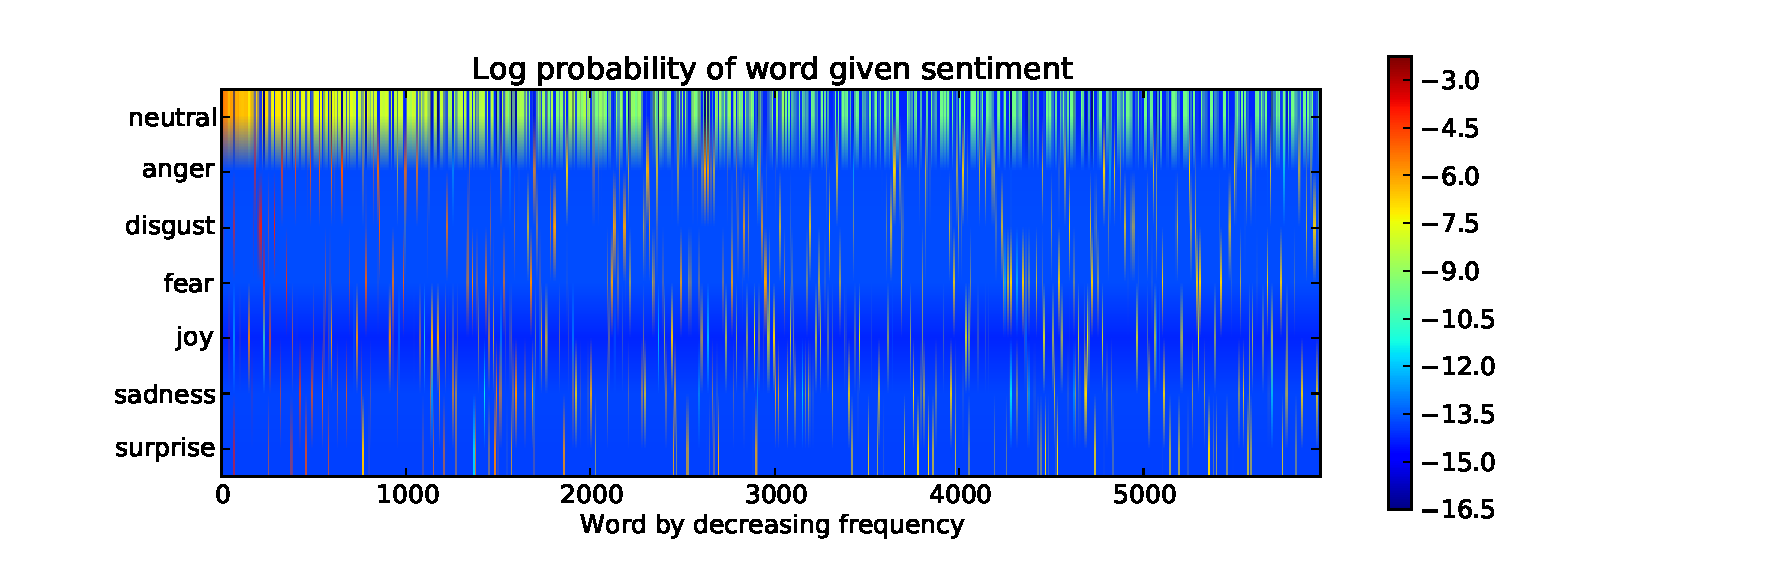
\includegraphics[width=\textwidth, trim=15mm 0mm 40mm 0mm, clip]{sentiment_heatmap}
\caption{Word mixing proportions in the SubjLDA model for each
sentiment for noconsensusonaname.tumblr.com. The bottom axes to
ordered by decreasing frequency. Most words belong to few sentiments.
\label{fig:sparse}}
\end{figure}

Furthermore, the model successfully chose sparse topic-word
and document-topic representations. Figure~\ref{fig:sparse} shows
the word mixing proportions for each sentiment for the blog
noconsensusonaname.tumblr.com.

\subsection{Evaluation}
For each model, we report the perplexity of the test set \citep{blei03}.
Intuitively, if probability model assigns high probabilities to
newly observed events, then the exponent term is large, so the
perplexity is low. The model is less ``surprised'' by the new
information and in fact already predicted something close. Since
perplexity is evaluated on a test set, lower perplexity implies
better generalization.
\begin{equation}
perp(D_{test}) = \exp{\left(-\frac{\sum_{d=1}^M \log{p(\mathbf{w}_d)}}{\sum_{d=1}^N N_d}\right)}
\end{equation}
where $\mathbf{w}_d$ denotes the sequence of words for document
$d$.

Our baseline is the labels from Wordnet-Affect and SentiWordNet
alone.  We must formulate this baseline as a generative model in
order to compute perplexity. We allow the baseline a trivial training
step to label each sentiment word in training corpus as it is able
to, and then for each sentiment $k$, compute its frequency $f_k$
in training corpus.  Then, for each word index $i$, we draw a
sentiment label $k_i$ with probability $f_{k_i} / V$, where $V$ is
the size of the corpus vocabulary. Next, draw a word $w_i$ from the
sentiment $k_i$'s list with probability $g_{w_i} / f_{k_i}$. The
likelihood of observing any one word is thus
\begin{equation} \label{eqn:base-likelihood}
\begin{aligned}
p(w) &= \sum_{k=1}^K p(w|k) p(k) \\
     &= \sum_{k=1}^K \frac{g_w}{V}
\end{aligned}
\end{equation}
provided $w$ exists in the lexicon. If not, then we simply assign
$p(w) = 1/V$. That is, we assume new words do not enter.

\subsection{Derivation of SubjLDA's Likelihood of New Data}
As Lin did not derive a conditional distribution for the per-document
likelihood of SubjLDA, so we derive it here. Given the above MAP
estimates of these model parameters, we simply marginalize over the
subjectivity labels $\mathbf{s}$ and sentiment labels $\mathbf{k}$.
SubjLDA assumes that given a document, per-sentences subjectivity
labels are drawn i.i.d., and given a sentence, per-word sentiment
labels are drawn i.i.d.

First, at the end of the Gibbs sampling, we obtain maximum a
posteriori estimates of the model parameters $\mathbf{\Pi}$,
$\mathbf{\Theta}$, and $\mathbf{\Phi}$ from the samples. This is
easy to do because each parameter is a matrix of multinomial
proportions, which we estimate by smoothing sample means with our
priors. We present Lin's results here~\citep{lin03}.

Let $\pi_{d,j}$ denote the probability that sentences in document
$d$ takes subjectivity $j$, $\theta_{d,m,k}$ denote the probability
that a word in sentence $m$ of document $j$ takes sentiment $k$,
and $\phi_{k,t}$ denote the probability a word of sentiment $k$ is
word $t$. Then the MAP estimates for our model parameters are
\begin{align}
\pi_{d,j}      &= \frac{N_{d,j} + \gamma}{N_d + K\gamma} \\
\theta_{d,m,k} &= \frac{N_{d,m,k} + \alpha_{s_{d,m},k}}{N_{d,m} + \sum_{j=1}^S \alpha_{s_{d,m},k}} \\
\phi_{k,t}     &= \frac{N_{k,t} + \beta_{k,t}}{N_k + \sum_{t=1}^V \beta_{k,t}}
\end{align}
where $N_{\mathbf{x}}$ denotes the count of all words matching
index $\mathbf{x}$, $S$ is the number of sentiments, and $V$ is the
vocabulary size.

There is one caveat: $\mathbf{\Theta}$ is a dummy variable,
parameterized by a document and sentence counts in the training
set. In the likelihood formula for new data, we analytically integrate
out $\Theta$ and perform our estimations from $\alpha$, reestimated
by maximum likelihood from the sampling results at the end of training.

Let $M$ denote the number of sentences in a document, $N_m$ denote
the number of words in sentence $m$, and $w_{m,n}$ denote the word
at position $n$ in sentence $m$. Then the likelihood of a new
document $\mathbf{w}$ is
\begin{equation} \label{eqn:subjlda-likelihood}
\begin{aligned}
P(\mathbf{w} | \mathbf{\Pi,\Theta,\Phi,\alpha,\beta,\gamma}) 
    &= \prod_{m=1}^M \sum_{l=1}^L \prod_{n=1}^N \sum_{k=1}^K \int P(w_{m,n} | k, \mathbf{\Phi} ) P( k | \theta ) P ( \theta | \alpha_l) d\theta \\
    &= \prod_{m=1}^M \sum_{l=1}^L \prod_{n=1}^N \sum_{k=1}^K \int \phi_{k,w_{m,n}} \theta_k \frac{\Gamma \left( \sum_{k=1}^K \alpha_{l,k} \right)}{\prod_{k=1}^K \Gamma(\alpha_{l,k})} \prod_{k=1}^K \theta_k^{\alpha_{l,k} - 1} d\mathbf{\theta} \\
    &= \prod_{m=1}^M \sum_{l=1}^L \prod_{n=1}^N \sum_{k=1}^K \phi_{k,w_{m,n}} \frac{\Gamma \left( \sum_{k=1}^K \alpha_{l,k} \right)}{\prod_{k=1}^K \Gamma(\alpha_{l,k})} \frac{\prod_{k'=1}^K \Gamma(\alpha_{l,k'} + \left[ k' = k \right])}{\Gamma \left( \sum_{k'=1}^K \alpha_{l,k'} + \left[ k' = k \right] \right)}
\end{aligned}
\end{equation}
where $[\cdot]$ are Iverson brackets. In the last line, we use the
fact that $P( k | \theta ) P ( \theta | \mathbf{\alpha}_l)$ is a
Dirichlet distribution with parameter $(\alpha_{l,1}, \ldots,
\alpha_{l,k} + 1, \ldots, \alpha_{l,K})$, so the integral evaluates
to 1 and we need only multiply the normalizing constants.

\subsection{Derivation LDA's Likelihood of New Data}
Since in LDA, $\theta$ is also a dummy variable that is valid only
for the documents in the training set, we also re-estimate the prior
$\alpha$ and then marginalize over $\theta$. The likelihood of a new
document $\mathbf{w}$ is
\begin{equation} \label{eqn:lda-likelihood}
\begin{aligned}
P(\mathbf{w} | \theta, \mathbf{\Phi}, \alpha, \beta )
 &= \prod_{n=1}^N \sum_{k=1}^K \int P(w_n | k, \mathbf{\Phi}) P(k | \theta) p(\theta | \alpha) d\theta \\
 &= \prod_{n=1}^N \sum_{k=1}^K \phi_{k,w_n} \frac{\prod_{k=1}^K \Gamma(\alpha_{k})}{\Gamma \left( \sum_{k=1}^K \alpha_{k} \right)} \frac{\prod_{k'=1}^K \Gamma(\alpha_{k'} + \left[ k' = k \right])}{\Gamma \left( \sum_{k'=1}^K \alpha_{k'} + \left[ k' = k \right] \right)}
\end{aligned}
\end{equation}

\subsection{Perplexity Results and Discussion}
Figure~\ref{tab:perp} shows that while SubjLDA achieved an order
of magnitude improvement in the medium (poetry) dataset, but actually
underperformed LDA on the small (prose) dataset. Both model so
substantially better than the baseline.

\begin{table}
\centering
\begin{tabular}{l c c c}
\bf Dataset & \bf Baseline & \bf LDA & \bf SubjLDA \\
\hline
thenatureofdaylight.tumblr.com & $3.067 \times 10^{23}$ & $2.494 \times 10^{-19}$ & $\mathbf{3.679 \times 10^{-18}} $ \\
noconsensusonaname.tumblr.com & $1.950 \times 10^{19}$ & $\mathbf{2.393 \times 10^{-17}}$ & $2.664 \times 10^{-17}$ \\
pantslessprogressive.com & 0 & 0 & 0 \\
\end{tabular}
\caption{Perplexity measures for each dataset and each model.\label{tab:perp}}
\end{table}


\begin{small}
\bibliographystyle{plainnat}
\bibliography{refs} 
\end{small}
\section*{Appendix: Post-Mortem}
While the results for this project could have been better, I've
certainly learned a lot from doing this work.

First, as described in the abstract, \emph{immature} really does
capture the state of the art in web sentiment analysis. Several
well-cited approaches, including \citep{mishne06, alm08, sood09}
employ elementary techniques. While these discriminative models
successfully classify these selected datasets, they give little
insight as to the dynamics of a single person's emotional state.
Thus, they are of less utility to, say, designing human-computer
interfaces to respond according to a user's emotions.

This is partially due to the nature of emotion: all emotions
are hidden variables because nobody can read your mind. So any
observations, textual, verbal, or physiological are necessarily
noise. Words are especially ambiguous at communicating emotion,
though they are the most easily accessible data. Nevertheless, good
classifications results for large supervised problems have been
achieved, a large number of which use SVMs. Sufficient data does
indeed overwhelm noise, and does not require much clever trickery
to tease out the relationships within the data. This was a lesson
often reiterated during class which I am learning by omission. But
conversely, if your data is too sparse, then no amount of nonlinear
Bayesian trickery may be able to save you.

I had hoped to find some work in the literature building psychological
or neurologically-based models for sentiment analysis, but alas
these hopes are a bit beyond the time for this field.

Second, I learned just how much of a pain it is to deal with all
but the most trivial of datasets. Many results were obtained with
a 8.1 million-post Livejournal corpus. I had wanted to compare my
my unsupervised approaches with a more typical SVM formulation.
Though many papers used this dataset, after hours of crawling the
web, I was unable to find a download for myself.

Other datasets were not trivial to acquire or use. Many required
filling out a registration form and waiting for days \citep{baccianella10}.
The data came in a hodge-podge of text formats, requiring lots of
crufy parsing code, a distraction from the real data-driven modelling.
Scraping your own textual data doesn't give you labels, preventing
access to supervised methods.
\end{document}

